\documentclass{beamer}
\mode<presentation>
\usepackage{amsmath}
\usepackage{amssymb}
\usepackage{mathtools}
\usepackage{listings}
\usepackage{graphicx}
\usepackage{hyperref}
\usetheme{Boadilla}
\usecolortheme{lily}

\setbeamertemplate{footline}{
  \leavevmode%
  \hbox{% 
    \begin{beamercolorbox}[wd=.9\paperwidth,ht=2.25ex,dp=1ex,left]{author in head/foot}%
      \hspace{1em} Arnav Makarand Yadnopavit
    \end{beamercolorbox}%
    \begin{beamercolorbox}[wd=.1\paperwidth,ht=2.25ex,dp=1ex,right]{author in head/foot}%
      \insertframenumber{} / \inserttotalframenumber\hspace*{2ex}
    \end{beamercolorbox}}%
}
\setbeamertemplate{navigation symbols}{}

\numberwithin{equation}{section}
\title{11.16.3.9: Probability of Complementary Events}
\author{EE24BTECH11007 - Arnav Makarand Yadnopavit}
\date{\today}

\begin{document}

\begin{frame}
\titlepage
\end{frame}

\section*{Outline}
\begin{frame}
\tableofcontents
\end{frame}

\section{Question}
\begin{frame}
\frametitle{Question}
If $\dfrac{1}{12}$ is the probability of an event, what is the probability of the event 'not A'?
\end{frame}

\section{Solution}
\subsection{Bernoulli Random Variable}
\begin{frame}
\frametitle{Bernoulli Random Variable}
Let us solve the problem using a Bernoulli random variable.

The Bernoulli R.V is defined as:
\begin{align}
	X_i = \begin{cases}
		0 & \text{not A}\\	
		1 & \text{A}	
	\end{cases}
\end{align}

The PMF of Bernoulli R.V is given by:
\begin{align}
  p_X(x) = \begin{cases}
    1-p & x = 0\\
    p & x = 1
  \end{cases}
\end{align}
\end{frame}

\subsection{Probability Calculation}
\begin{frame}
\frametitle{Probability Calculation}
\begin{itemize}
    \item The probability of $ A $ occurring is given as $ P(A) = \dfrac{1}{12} $.  
    Therefore, $ p_X(1) = P(A) = \dfrac{1}{12} $.

    \item The probability of the complement of $ A $ (denoted as "not $ A $") is $ P(A^\prime) = p_X(0) $. Using the rule of complementary probabilities:
    \[
    P(A^\prime) = 1 - P(A).
    \]

    \item Substitute $ P(A) = \dfrac{1}{12} $ into the equation:
    \[
    P(A^\prime) = 1 - \dfrac{1}{12} = \dfrac{11}{12}.
    \]
\end{itemize}
\end{frame}

\subsection{PMF of Bernoulli R.V}
\begin{frame}
\frametitle{PMF of Bernoulli R.V}
Thus, the probabilities for the Bernoulli random variable $ X $ are:
\begin{align}
  p_X(x) = \begin{cases}
    \dfrac{11}{12} & x = 0\\\\
    \dfrac{1}{12} & x = 1
  \end{cases}
\end{align}
Hence, the probability of the event 'not A' is $\dfrac{11}{12}$.\\
Code for finding probability using computational methods can be found at below link\\
\url{https://github.com/ArnavYadnopavit/EE1003/tree/main/ncert/11.16.3.9/codes}
\end{frame}

\section{Stem Plot of the PMF}
\begin{frame}
\frametitle{Stem Plot of the PMF}
Below is the stem plot for the PMF of the Bernoulli random variable:
\begin{figure}[h]
    \centering
    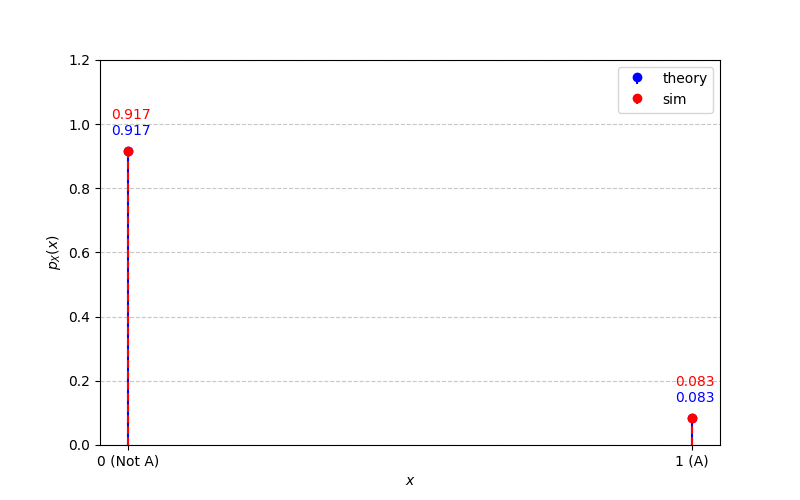
\includegraphics[width=0.8\linewidth]{figs/fig.png}
\end{figure}
\end{frame}

\end{document}
